% This template is used for pandoc
\documentclass[10pt]{ctexart}

\def\university{Harbin Institute of Technology}
\def\team{Dolls in Pseudo Paradise}
\def\season{2024-2025}

\usepackage{amsmath, amssymb}
\usepackage{graphicx}
\usepackage{float}
\usepackage{hyperref}

% ==================== Begin     Page ====================
%%%%%% fix pandoc
\providecommand{\tightlist}{\setlength{\itemsep}{0pt}\setlength{\parskip}{0pt}}
\newcommand{\passthrough}[1]{#1}

\usepackage[a4paper, includehead, headsep=0.1in, left=0.4in, right=0.1in, top=0.1in, bottom=0.1in, landscape]{geometry}
\ctexset{
    section = {
        beforeskip = { 1.5ex plus 1ex minus .2ex },
        afterskip  = { 1.3ex plus .2ex }
    },
    subsection = {
        beforeskip = { 1.25ex plus 1ex minus .2ex },
        afterskip  = { 0.5ex plus .2ex }
    },
    subsubsection = {
        beforeskip = { 1.25ex plus 1ex minus .2ex },
        afterskip  = { 0.5ex plus .2ex }
    },
}

% Three columns & landscape to make the code tight
\usepackage{multicol}
\setlength{\columnsep}{30pt}

% ==================== Begin     Font ====================
\usepackage{fontspec}
\setmonofont{FiraCode-Regular.ttf}[
    Path = utils/,
    BoldFont = FiraCode-Bold.ttf,
    ItalicFont = FiraCode-Light.ttf,
    BoldItalicFont = FiraCode-Medium.ttf,
    Contextuals=Alternate           % Activate the calt feature
]

\setCJKmainfont{SourceHanSerif-Regular.otf}[
    Path = utils/,
    BoldFont = SourceHanSans-Regular.otf,
    ItalicFont = SourceHanSerif-Light.otf
]

\newCJKfontfamily[jinwen]\jinwen{DFJinwen-W3}[
    Path = utils/,
    Extension = .otf,
]

% ==================== Begin   Header ====================
\usepackage{fancyhdr}
\usepackage{zref-totpages}
\usepackage{epigraph}
\pagestyle{fancy}
\fancyhf{} % Clear up default styles

\setlength{\headheight}{12.08003pt}

% Header Left: University + team name
\fancyhead[L]{\university -- \textit{\team}}

% Header Center: Section
\fancyhead[C]{\leftmark}

% Header Right: Page number
\fancyhead[R]{Page \thepage\ of \ztotpages}

% Header line
\renewcommand{\headrulewidth}{0.4pt}

%%%%%% Main Content

\usepackage{xcolor}
\usepackage{listings, lstfiracode} % https://ctan.org/pkg/lstfiracode

% Color Palletes from Gihub
\lstset{
  language=[11]C++,
  basicstyle    = \ttfamily\small\color[HTML]{24292E},
  style=FiraCodeStyle,   % Use predefined FiraCodeStyle
  keywordstyle    =\color[HTML]{D73A49}\bfseries,
  commentstyle    =\color[HTML]{6A737D},
  numberstyle     =\color[HTML]{005CC5}\bfseries\sffamily,
  stringstyle     =\color[HTML]{032F62}\bfseries,
  tabsize = 2,
  breaklines,
  basewidth={0.6em, 0.5em},
  breakindent = 1.1em,
  columns = fixed,
  numbers = left,
  frame = single,
  lineskip=-1pt
}

% from https://github.com/4thcalabash/code_library/blob/master/tex/format.tex
% an amazing script
% converts an line-number to arbitrary string
\let\othelstnumber=\thelstnumber
\def\createlinenumber#1#2{
    \edef\thelstnumber{%
        \unexpanded{%
            \ifnum#1=\value{lstnumber}\relax
             \tt #2%
            \else}%
        \expandafter\unexpanded\expandafter{\thelstnumber\othelstnumber\fi}%
    }
    \ifx\othelstnumber=\relax\else
      \let\othelstnumber\relax
    \fi
}

% Only 1 and 2 level
\setcounter{tocdepth}{2}

\begin{document}

\begin{titlepage}
    \thispagestyle{empty}

    \vspace*{-1cm}

    \hfill
    \parbox{0.5\textwidth}{
        \epigraph{
            \textsf {Our village of honest men originally consisted of only eight people.} \\
            \textsf {We all picked up and moved to a mountain in the east. Two years of honest and boring daily life passed us by.} \\
            \textsf {One day, one of us found a little hole by a peach tree.} \\
            \textsf {Yes, after that we wandered into this paradise.} \\
            \textsf {And right away, I quit being human.}
        }{\textit{--- Dolls in Pseudo Paradise}}
    }
    \hspace{0.5cm}

    \vfill
    
    \begin{center}
        \Huge {\jinwen 蓬莱人形}算法模板库 \\
        \huge {\textsc{Reference Document} for \textsl{\team}}
    \end{center}

    \vspace*{2cm}

    \begin{figure}[htbp]
        \centering
        \begin{minipage}[c]{0.25\textwidth}
            \centering
            
\includegraphics[width=6cm]{utils/images/hit-logo.png}
        \end{minipage}
        \hspace{1cm}
        \begin{minipage}[c]{0.25\textwidth}
            \centering
            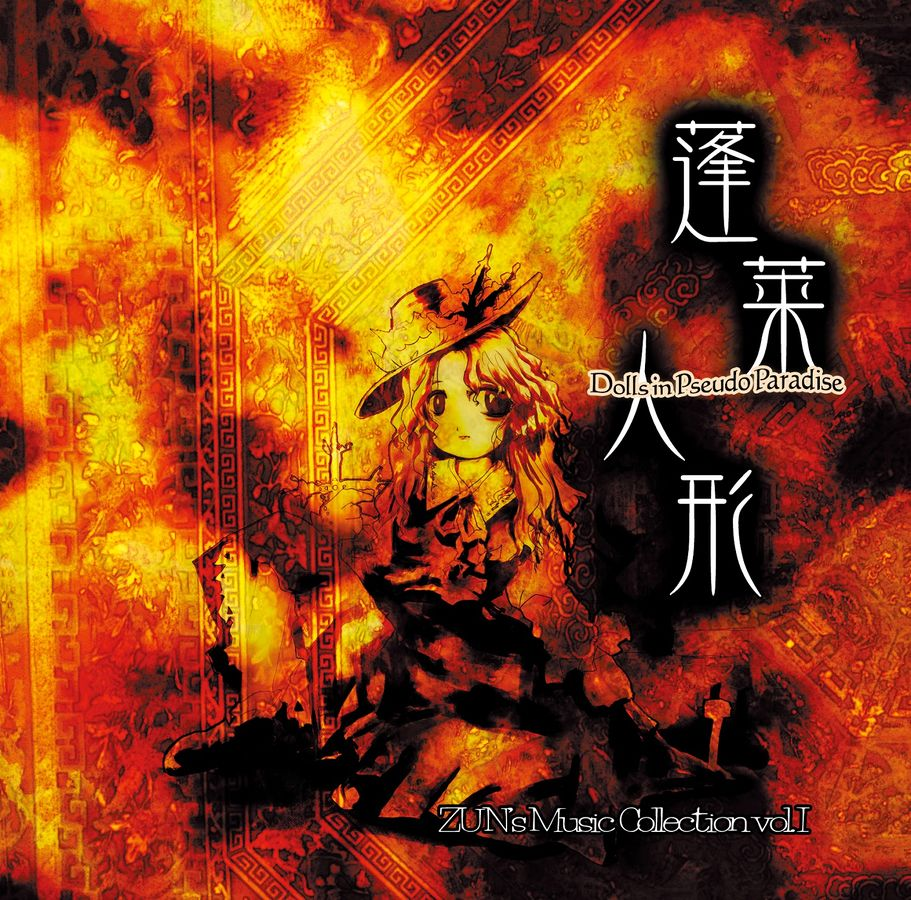
\includegraphics[width=6cm]{utils/images/hourai.jpg}
        \end{minipage}
        \hspace{1cm}
        \begin{minipage}[c]{0.25\textwidth}
            \centering
            
\includegraphics[width=6cm]{utils/images/icpc.png}
        \end{minipage}
    \end{figure}

    \vfill

    \begin{center}
        \Large \color{darkgray} \season \\
        \Large \color{darkgray} \university
    \end{center}

    \vspace*{1cm}
\end{titlepage}

\newpage

\begin{multicols}{3}
    \setcounter{page}{1}

    \tableofcontents
    
    $body$
\end{multicols}

\end{document}